
\section{Ablation Studies} \label{sec5}
Although we have demonstrated extremely strong empirical results, the results presented so far have not isolated the specific contributions from each aspect of the BERT framework. In this section, we perform ablation experiments over a number of facets of BERT in order to better understand their relative importance.

	\subsection{Effect of Pre-training Tasks} \label{sec5.1}
	One of our core claims is that the deep bidirectionality of BERT, which is enabled by masked LM pre-training, is the single most important improvement of BERT compared to previous word. To give evidence for this claim, we evaluate two new models which use the exact same pre-training data, fine-tuning scheme and Transformer hyperparameters as $\rm BERT_{BASE}$:
	
		\begin{enumerate}
			\item \textbf{No NSP}: A model which is trained using the ``masked LM" (MLM) but without the ``next sentence prediction" (NSP) task.
			\item \textbf{LTR \& NO NSP}: A model which is trained using a Left-to-Right (LTR) LM, rather than an MLM. In this case, we predict every input word and do not apply any masking. The left-only constraint was also applied at fine-tuning, because we found it is always worse to pre-train with left-only-context and fine-tune with bidirectional context. Additionally, this model was pre-trained without the NSP task. This is directly comparable to OpenAI GPT, but using our larger training dataset, our input representation, and our fine-tuning scheme.
		\end{enumerate}
	
	Results are presented in Table \ref{tab5}. We first examine the impact brought by the NSP task. We can see that removing NSP hurts performance significantly on QNLI, MNLI, and SQuAD. These results demonstrate that our pre-training method is critical in obtaining the strong empirical results presented previously.
	
	Next, we evaluate the impact of training bidirectional representations by comparing ``No NSP'' to ``LST \& No NSP''. The LTR model performs worse than the MLM model on all tasks, with extremely large drops on MRPC and SQuAD. For SQuAD it is intuitively clear that an LTR model will perform very poorly at span and token prediction, since the token-level. hidden states have no right-side context. For MRPC is unclear whether the poor performance is due to the small data size of the nature of the task, but we found this poor performance to be consistent across a full hyperparameters sweep with many random restarts. 
	
	In order make a good faith attempt at strengthening the LTR system, we tried adding a randomly initialized BiLSTM on top of it for fine-tuning. This does significantly improve results on SQuAD, but the results are still far worse than the pre-trained bidirectional models. It also hurts performance on all four GLUE tasks.
	
	\begin{table}[b]
	\centering
	\resizebox{\columnwidth}{!}{
	\begin{tabular}{@{}lccccc@{}} % remove padding in table two sides
	\toprule[0.11em] % control width of rule
	\multirow{3}{*}{Tasks} & \multicolumn{5}{c}{Dev Set} \\
	& MNLI-m  & QNLI  & MRPC & SST-2 & SQuAD  \\
	& (Acc) & (Acc) & (Acc) & (Acc) & (F1) \\
	\midrule[0.07em]
	$\rm BERT_{BASE}$ & 84.4 & 88.4 & 86.7 & 92.7 & 88.5 \\
	No NSP & 83.9 & 84.9 & 86.5 & 92.6 & 87.9 \\
	LTR \& No NSP & 82.1 & 84.3 & 77.5 & 92.1 & 77.8 \\
	\quad+ BiLSTM & 82.1 & 84.1 & 75.7 & 91.6 & 84.9 \\
	\bottomrule[0.11em]
	\end{tabular}}
	\caption{Ablation over the pre-training tasks using the BERTBASE architecture. ``No NSP'' is trained without the next sentence prediction task. ``LTR \& No NSP'' is trained as a left-to-right LM without the next sentence prediction, like OpenAI GPT. ``+ BiLSTM” adds a ran- domly initialized BiLSTM on top of the “LTR + No NSP'' model during fine-tuning.}
	\label{tab5}
	\end{table}
	
	We recognize that it would also be possible to train separate LTR and RTL models and representation token as the concatenation of the two models, as ELMo does. However: (a) this is twice as expensive as a single bidirectional model; (b) this is non-intuitive for tasks like QA, since the RTL model would not be able to condition the answer on the question; (c) this it is strictly less powerful than a deep bidirectional model, since a deep bidirectional model could choose to use either left or right context. 
		
	\subsection{Effect of Model Size} \label{sec5.2}
	In this section, we explore the effect of model size on fine-tuning task accuracy. We trained a number of BERT models with a differing number of layers, hidden units, and attention heads, while otherwise using the same hyperparameter and training procedure as described previously.
	
	Results on selected GLUE tasks are shown in Table \ref{tab6}. In this table, we report the average Dev Set accuracy from 5 random restarts of fine-tuning. We can see that larger models lead to a strict accuracy improvement across all four datasets, even for MRPC which only has 3600 labeled training examples, and is substantially different from the pre-training tasks. It is also perhaps surprising that we are able to achieve such significant improvements on top of models which are already quite large relative to the existing literature. For example, the largest Transformer explored in \citep{Ashish2017} is (L=6, H=1024, A=16) with 100M parameters for the encoder, and the largest Transformer we have found in the literature is (L=64, H=512, A=2) with 235M parameters \citep{Rami2018}. By contrast, $\rm BERT_{BASE}$ contains 100M parameters and $\rm BERT_{LARGE}$ contains 340M parameters.
	
	\begin{table}[b]
	\centering
	\resizebox{\columnwidth}{!}{
	\begin{tabular}{@{}rrrcccc@{}}
	\toprule[0.11em]
	\multicolumn{4}{l}{Hyperparams} & \multicolumn{3}{c}{Dev Set Accuracy} \\
	\midrule[0.07em]
	\#L & \#H & \#A & LM(ppl) & MNLI-m & MRPC & SST-2 \\
	3 & 768 & 12 & 5.84 & 77.9 & 79.8 & 88.4 \\
	6 & 768 & 3 & 5.24 & 80.6 & 82.2 & 90.7 \\
	6 & 768 & 12 & 4.68 & 81.9 & 84.8 & 91.3 \\
	12 & 768 & 12 & 3.99 & 84.4 & 86.7 & 92.9 \\
	12 & 1024 & 16 & 3.54 & 85.7 & 86.9 & 93.3 \\
	24 & 1024 & 16 & 3.23 & 86.6 & 87.8 & 93.7 \\
	\bottomrule[0.11em]
	\end{tabular}}
	\caption{Ablation over BERT model size. \#L = the number of layers; \#H = hidden size; \#A = number of at- tention heads. ``LM (ppl)'' is the masked LM perplexity of held-out training data.}
	\label{tab6}
	\end{table}
	
	It has been known for many years that increasing the model size will lead to continual improvements on large-scale tasks such as machine translation and language modeling, which is demonstrated by the LM perplexity of held-out training data shown in Table \ref{tab6}. However, we believe that this is the first work to demonstrate that scaling to extreme model sizes also leads to large improvements on every small scale tasks, provided that the model has been sufficiently pre-trained.
	
	\subsection{Effect of Number of Training Steps} \label{sec5.3}
	Figure \ref{fig4} presents MNLI Dev accuracy after fine-tuning from a checkpoint that has been pre-trained for $k$ steps. This allows us to answer the following questions:
	
	\begin{enumerate}
		\item Question: Does BERT really need such a large amount of pre-training (128000 words/batch * 1000000 steps) to achieve high fine-tuning accuracy? \\
			Answer: Yes, $\rm BERT_{BASE}$ achieves almost 1.0\% additional accuracy on MNLI when trained on 1M steps compared to 500k steps.
		\item Question: Does MLM pre-training converge slower than LTR pre-training, since only 15\% of words are predicted in each batch rather than every word? \\
			Answer: The MLM model does converge slightly slower than the LTR model. However, in terms of absolute accuracy the MLM model begins to outperform the LTR model almost immediately.
	\end{enumerate}
	
	
	\subsection{Feature-based Approach with BERT} \label{sec5.4}
	
	% fig4
	\begin{figure}[!b]
	\centering
	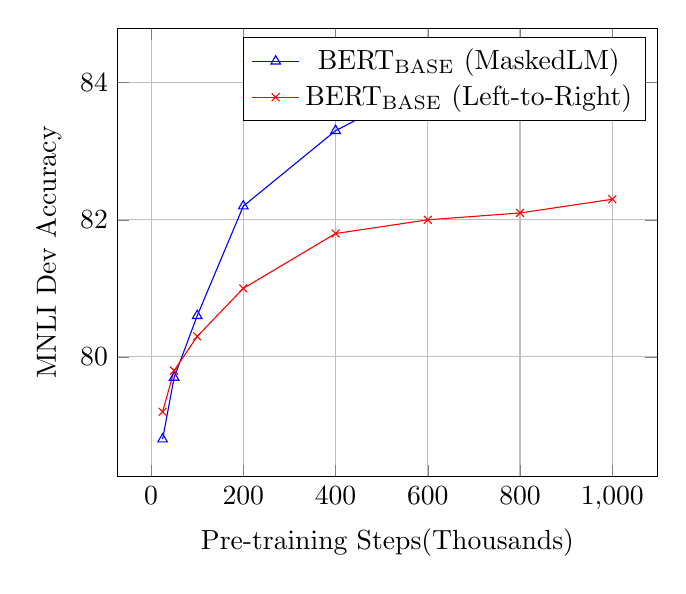
\begin{tikzpicture} \label{fig4}
		\begin{axis}[
			xlabel=Pre-training Steps(Thousands),
			ylabel=MNLI Dev Accuracy,
			grid=major]
		% blue 
		\addplot[color=blue, mark=triangle] coordinates {
			(25, 78.8)
			(50, 79.7)
			(100, 80.6)
			(200, 82.2)
			(400, 83.3)
			(600, 84)
			(800, 84.15)
			(1000, 84.25)
		};
		\addlegendentry{$\rm BERT_{BASE}$ (MaskedLM)};
		% red
		\addplot[color=red,mark=x] coordinates {
			(25, 79.2)
			(50, 79.8)
			(100, 80.3)
			(200, 81)
			(400, 81.8)
			(600, 82)
			(800, 82.1)
			(1000, 82.3)
		};
		\addlegendentry{$\rm BERT_{BASE}$ (Left-to-Right)};
	
		\end{axis}
	\end{tikzpicture}
	\caption{Ablation over number of training steps. This shows the MNLI accuracy after fine-tuning, starting from model parameters that have been pre-trained for k steps. The x-axis is the value of $k$.}
	\end{figure}
	
	\begin{table}[hbp]
	\centering
	\begin{tabular}{@{}lc@{}}
	\toprule[0.11em]
	Layers & Dev F1 \\
	\midrule[0.07em]
	Finetune All & 96.4 \\
	\midrule[0.07em]
	First Layer (Embeddings) & 91.0 \\
	Second-to-Last Hidden 95.6 \\
	Last Hidden & 94.9 \\
	Sum Last Four Hidden & 95.9 \\
	Concat Last Four Hidden & 96.1 \\
	Sum All 12 Layers & 95.5 \\
	\bottomrule[0.11em]
	\end{tabular}
	\caption{Ablation using BERT with a feature-based ap- proach on CoNLL-2003 NER. The activations from the specified layers are combined and fed into a two-layer BiLSTM, without backpropagation to BERT.}
	\label{tab7}
	\end{table}

	\begin{table}
	\end{table}
	
	
	
	
	
	
	
	
	
	